We used our approach on the following use cases:

\subsection{\textbf{Regression Comparison}}
    A software company is releasing its new version of software with several new features. The performance regressions tests did not find problems and the unitary tests were accepted. Some weeks after the release, the users started to complain about performance issues in one of the features.
    
\textbf{Approach:} 
    Our approach was to run the software several times on the previous and in the current version of the software. Then classified the data using our approach in slow and fast executions. 
        
\textbf{Results:}
    We were able to find that inline function addition on the feature increased the number of cache misses and therefore increased the elapsed time of this application. On the source code the inline functions could be seen as difference although the developers thought that this would improve performance and not decrease it.
    
    \lstset{language=C++,
            backgroundcolor=\color{black!2}, % set backgroundcolor
            basicstyle=\ttfamily\footnotesize,% basic font setting
            keywordstyle=\color{blue}\ttfamily,
            stringstyle=\color{red}\ttfamily,
            commentstyle=\color{gray}\ttfamily,
            morecomment=[l][\color{gray}]{\#}
    }
    \begin{lstlisting}[caption={Example of Code for inline}, label=pseudo:case-inline, captionpos=b]
    //header file
    #ifndef EXAMPLE_H
    #define EXAMPLE_H
    /*  
     *  Function included in multiple source
     *  files must be inline 
     */
    inline int sum(int a, int b) {
        return a + b;
    }
    inline void tolower(char* str) {
        for(int i = 0; str[i]; i++)
          str[i] = tolower(str[i]);
    }
    #endif
    \end{lstlisting}
    
    
    Using a comparative approach of the groups we could see the difference of the metrics withing them. Comparing the groups of inline functions and the groups without inline, we verified that the inline groups comparatively to their respective groups of non-inline, had a significant amount of cache misses. Concluding that cache misses was the essence of the differences as shown in Table \ref{tab:table}.
    
\begin{table}[h]
    \centering
    \caption{Grouping results relating the cache misses with the slow executions groups}
    \label{tab:table}
    \begin{tabular}{ll}
        
        \multicolumn{2}{c}{Executions}                        \\ \hline
        Fast group                & Slow group                \\ \hline
        mean of 2500 cache misses & mean of 6500 cache misses \\ \hline
    \end{tabular}
\end{table}


\subsection{\textbf{Page Faults Interference}}
	A software company deployed several new packages in its software. Those changes included a function implementation, which executes several times the process of writing in a buffer. This problem usually occurs  after several sub-sequential executions.
Performance tools were able to discover a performance impact on these new changes but it is not possible to track specifically which commit caused the impact. The company would need to run specific Linux commands to find the reason for this problem or reproduce several performance tests with each commit. This scenarios was taken from \cite{essentials} also related to Microsoft bug in \cite{microsoft_bug}. 

\textbf{Approach:}
    Our approach was to instrument the code and to run the software several times on the previous and in the current version of the software. Then classify the data using our approach in slow and fast executions and compare it in a pair-wise comparision. Although the auto-grouping gave more groups, i.e. reduction of ten to two groups of comparison, the aim was to specific compare two groups of executions: fast and slow group.


  
\textbf{Results:}
    The tree generated had branches with fast and slow executions aggregated together. The nodes recorded the several performance metrics including the instructions, cache misses and page faults. We were able to find that page faults extra addition on the feature decreased the performance. On slow executions, the page faults were classified on other group. The tool revealed the association, and we can conclude that the program triggers more page faults specifically after several executions.
	On the source code, the change on the buffer was an array that was implemented using a row major storage scheme and caused an addition of about 16.384 page faults.
     The company was not able to track this problem before, because of the prefetching algorithms influence of the executions. This technique is used on the microprocessor architecture to speedup the instructions. 
    %  The Figure \ref{fig:case1} (\textcolor{red}{ADD TRACECOMPASS PLOT HERE}), is a CCTView result that expose this difference from several runs.

 The code in highlight shows the difference on the array coding that created the page faults difference. This code was taken from \cite{essentials}.
% \lstset{language=C++,
%                 backgroundcolor=\color{black!2}, % set backgroundcolor
%                 basicstyle=\ttfamily\footnotesize,% basic font setting
%                 keywordstyle=\color{blue}\ttfamily,
%                 stringstyle=\color{red}\ttfamily,
%                 commentstyle=\color{gray}\ttfamily,
%                 morecomment=[l][\color{gray}]{\#}
% }
% \begin{lstlisting}[caption={Page fault interference - code changes}, label=pseudo:page-faults, captionpos=b]

%     //Considering 128 words/page
%     int i, j;
%     int data[128][128]; 
%     // original version
%     for(i = 0; i < 128; i++)
%         for(j = 0; j < 128; j++)
%             data[i][j] = 0;
%     // new version
%     for(j = 0; j < 128; j++)
%         for(i = 0; i < 128; i++)
%             data[i][j] = 0;

% \end{lstlisting}
    
\lstdefinelanguage{diff}{
  sensitive=true,
  % diff command line
  morecomment=[f][\color{gray}][0]{diff},
  % commit identifiers for git diff
  morecomment=[f][\color{gray}][0]{index},
  % hunk location/line numbers for unified format
  morecomment=[f][\color{blue}][0]{@@},
  % hunk location/line numbers for context format
  morecomment=[f][\color{magenta}][0]{***},
  % changed line for context format
  morecomment=[f][\color{violet}][0]{!},
  % deleted lines for unified format
  morecomment=[f][\color{red!60!black}][0]-,
  % added lines for unified format
  morecomment=[f][\color{green!60!black}][0]+,
  % file name and time stamp old file
  morecomment=[f][\color{magenta}][0]{---},
  % file name and time stamp new file
  morecomment=[f][\color{magenta}][0]{+++},
  % Binary files ... differ
  morecomment=[f][\color{gray}][0]{Binary},
  % Only in ...: file.txt
  morecomment=[f][\color{gray}][0]{Only},
  % old mode ...
  morecomment=[f][\color{gray}][0]{old},
  % new mode ...
  morecomment=[f][\color{gray}][0]{new},
  % rename from/to ...
  morecomment=[f][\color{gray}][0]{rename},
  % similarity index ...%
  morecomment=[f][\color{gray}][0]{similarity},
  % deleted file mode ...%
  morecomment=[f][\color{gray}][0]{deleted},
  % hunk separator for context format
  morecomment=[f][\color{magenta}][0]{***************},
  % deleted lines for normal format
  morecomment=[f][\color{red!60!black}][0]<,
  % added lines for normal format
  morecomment=[f][\color{green!60!black}][0]>,
  % line number specifier for normal format
  morecomment=[f][\color{blue}][0]{0},
  % line number specifier for normal format
  morecomment=[f][\color{blue}][0]{1},
  % line number specifier for normal format
  morecomment=[f][\color{blue}][0]{2},
  % line number specifier for normal format
  morecomment=[f][\color{blue}][0]{3},
  % line number specifier for normal format
  morecomment=[f][\color{blue}][0]{4},
  % line number specifier for normal format
  morecomment=[f][\color{blue}][0]{5},
  % line number specifier for normal format
  morecomment=[f][\color{blue}][0]{6},
  % line number specifier for normal format
  morecomment=[f][\color{blue}][0]{7},
  % line number specifier for normal format
  morecomment=[f][\color{blue}][0]{8},
  % line number specifier for normal format
  morecomment=[f][\color{blue}][0]{9},
}[comments]
\lstset{language=diff}
\begin{lstlisting}[caption={Page fault interference - code changes}, label=pseudo:page-faults, captionpos=b]

    //Considering 128 words/page
    int i, j;
    int data[128][128]; 
    for(j = 0; j < 128; j++)
        for(i = 0; i < 128; i++)
-            data[i][j] = 0;
+            data[j][i] = 0;
\end{lstlisting}

\subsection{\textbf{Cache Optimization in Server Application}}
    A server application using a very known PHP content-management framework Drupal, caches requested data to improve the time access of its content. However, we observed that after 100 requests, the request response time was increased dramatically. Although, no change been introduced in software or hardware system, which is very difficult to analyze, Figure \ref{fig:server-time-series}.\\
    Drupal implement a caching mechanism which intend to improve the performance of access. In some executions we noticed the influence of the compile time, which is a infrequent behavior of php.
    
\textbf{Approach:}
    First we instrumented PHP and Apache server, to be able to measure its behavior. Our approach was to execute several times a request for a server. While running it, we recorded the tracing data. Then, we executed our clustering analysis and classified the data in several groups, which we can study their behavior. Using this approach is possible to track infrequent issues in the execution, that is, if we have one or two groups that a total different behavior, it is possible to study their properties.
    
\textbf{Results:}
    From the collected data we applied the auto-classification, which showed mainly two groups of comparison. The solution was able to display that on the fast group no time was spent on caching or php compilation time. However, on slow executions, there was a considerable time spent on compilation time and cache time, about 49\%, see black bars in Figure \ref{fig:server-time-series}. The approach was able to show impact of disk access overhead related to caching mechanism.\\
    The cache will be full and it will be flushed and built again. So specifically on each 100 request the server will spend more time than on the previous requests as shown in Figure \ref{fig:server-time-series}. The results are summarized in the Figure \ref{fig:groups_php}.
    
        
    \begin{figure}[h]
      \centering
        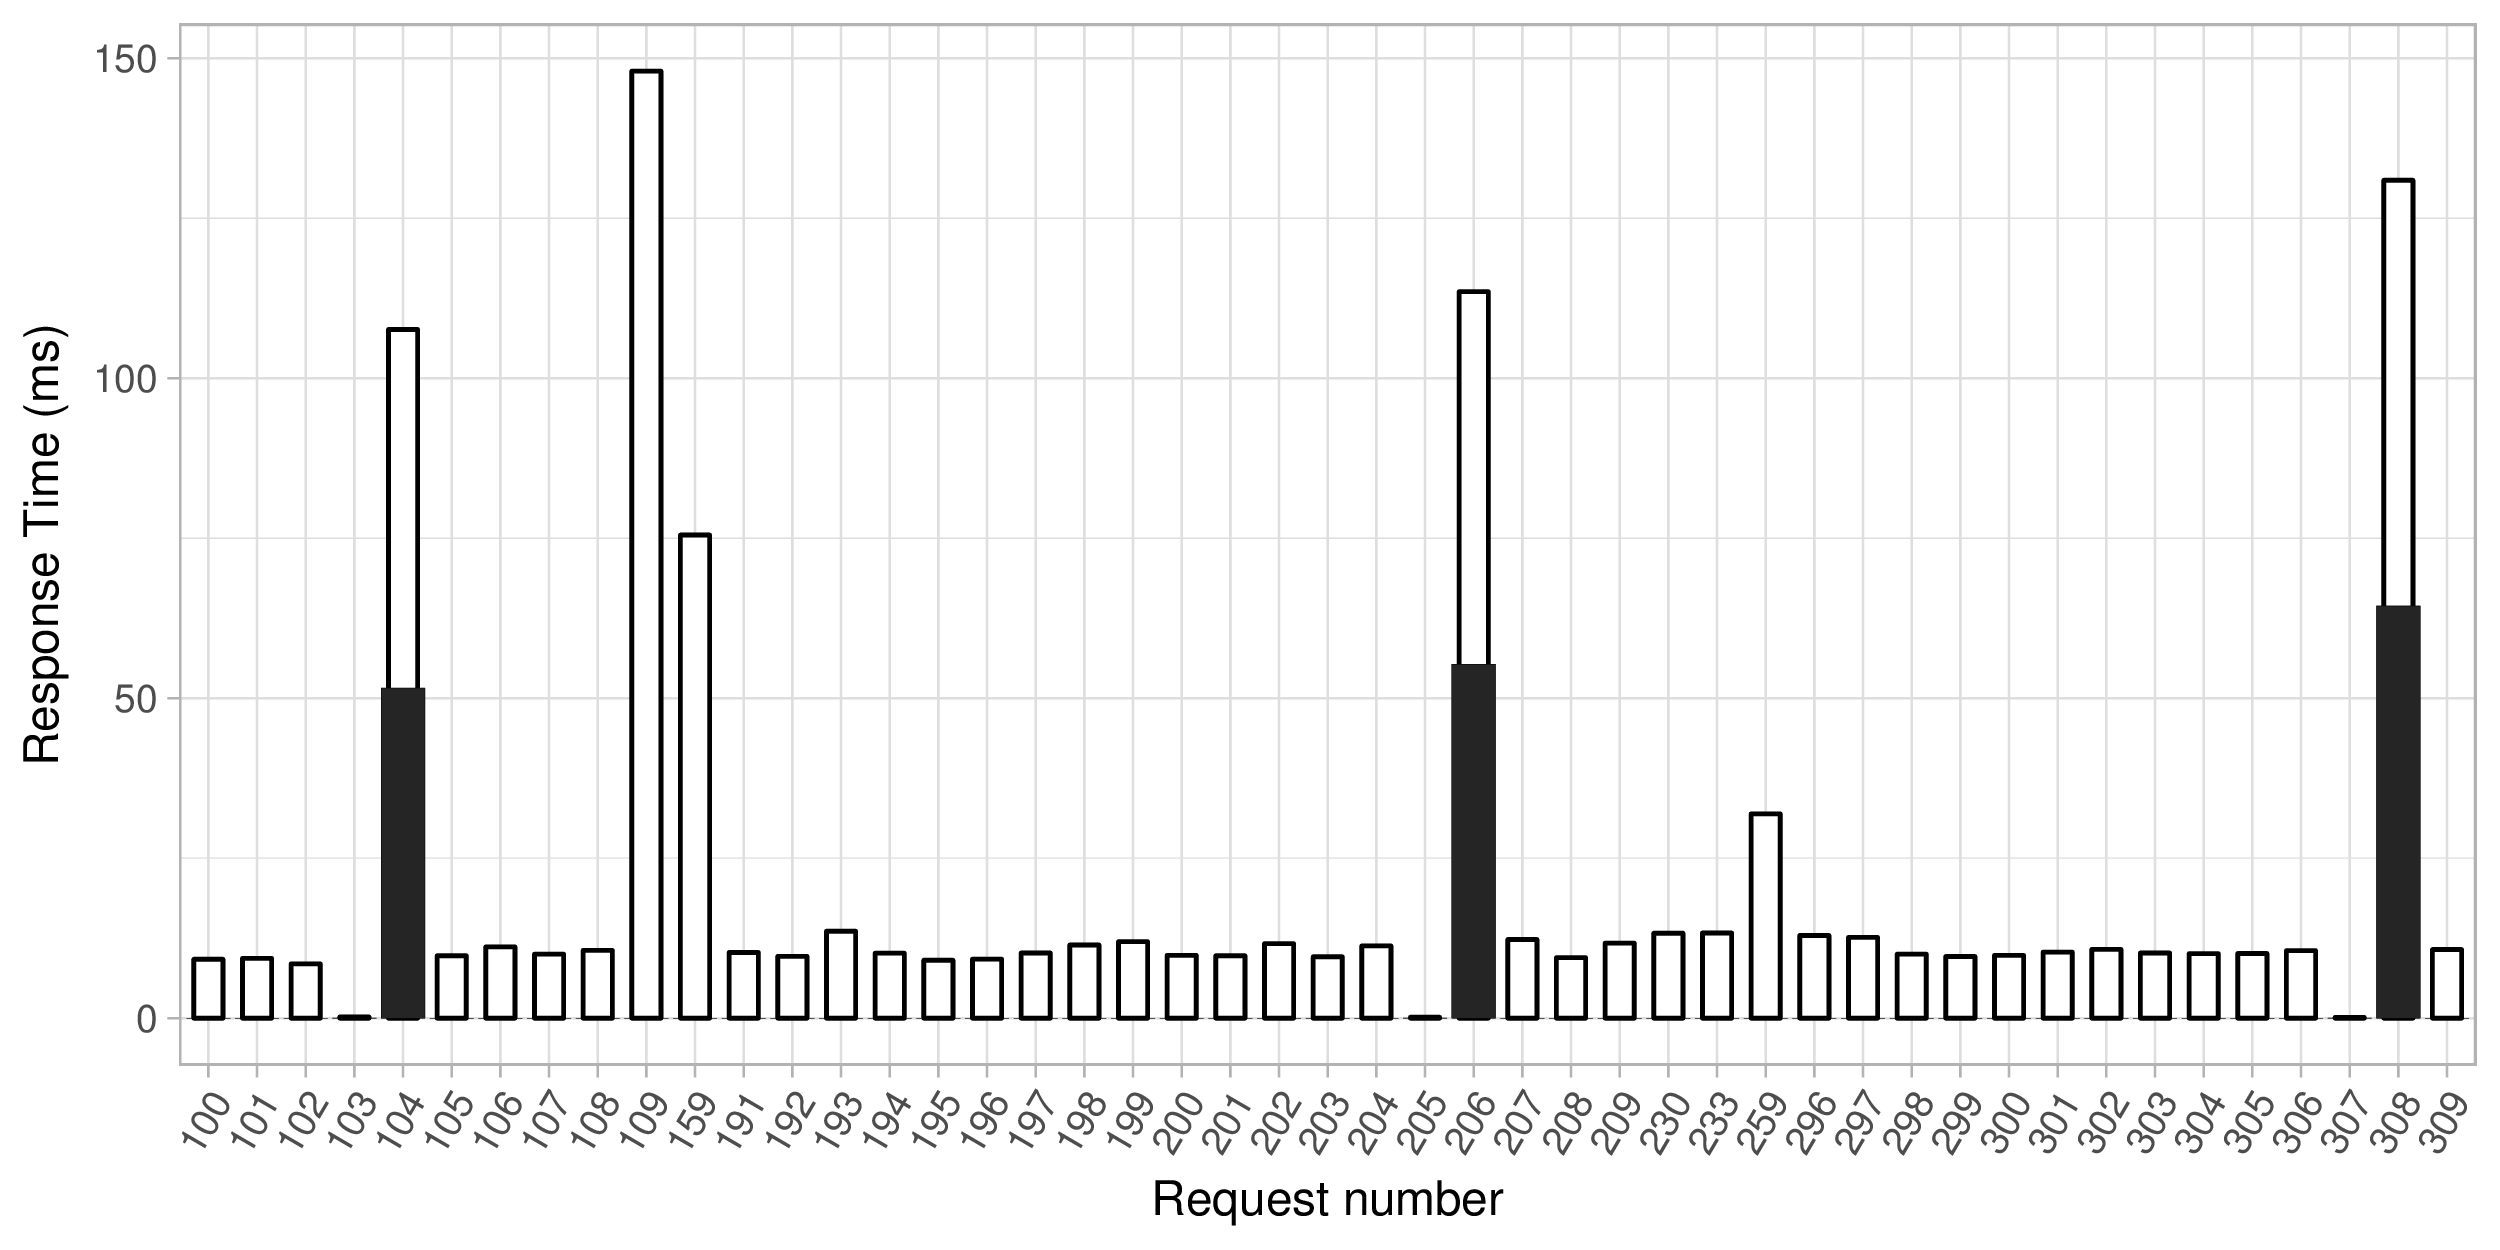
\includegraphics[width=1.0\textwidth]{figures/server-time-series-bar.png}
        \caption{Overhead introduced by I/O for caching on each 100 of requests, The white bars are the request response time and the dark bars represent the PHP compilation time}
        \label{fig:server-time-series}
    \end{figure}
    
    
    \begin{figure}[h]
    \centering
        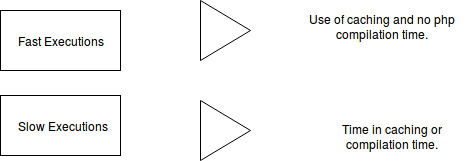
\includegraphics[width=0.50\textwidth]{figures/groups_results.jpg}
         \caption{Difference on the groups}
         \label{fig:groups_php}
     \end{figure}
    
% \subsection{\textbf{Task Scheduling Overhead}}
%     JSON is a lightweight data-interchange format. It can represent numbers, strings, ordered sequences of values, and collections of name/value pairs.

%     JsonCpp is a C++ library that allows manipulating JSON values, including serialization and deserialization to and from strings. It can also preserve existing comment in unserialization/serialization steps, making it a convenient format to store user input files.
    
%     Executing several times the reading from json file, some of the executions have a different time to read those files.    
    
% \textbf{Approach:}
%     Our approach was to run the software several times and run the clustering technique then compare the metrics between the groups.
%     The auto-grouping technique showed more than 10 groups to be compared, but only a few were taken in consideration.
    
% \textbf{Results:}
%     The solution showed differences on the branches of the tree and was able to display the relation with scheduler switches and the performance of this task, this would impact directly on a real task. All the tasks that took more time were related to task scheduling and switches.
    
\begin{figure*}[t!]
  \centering
    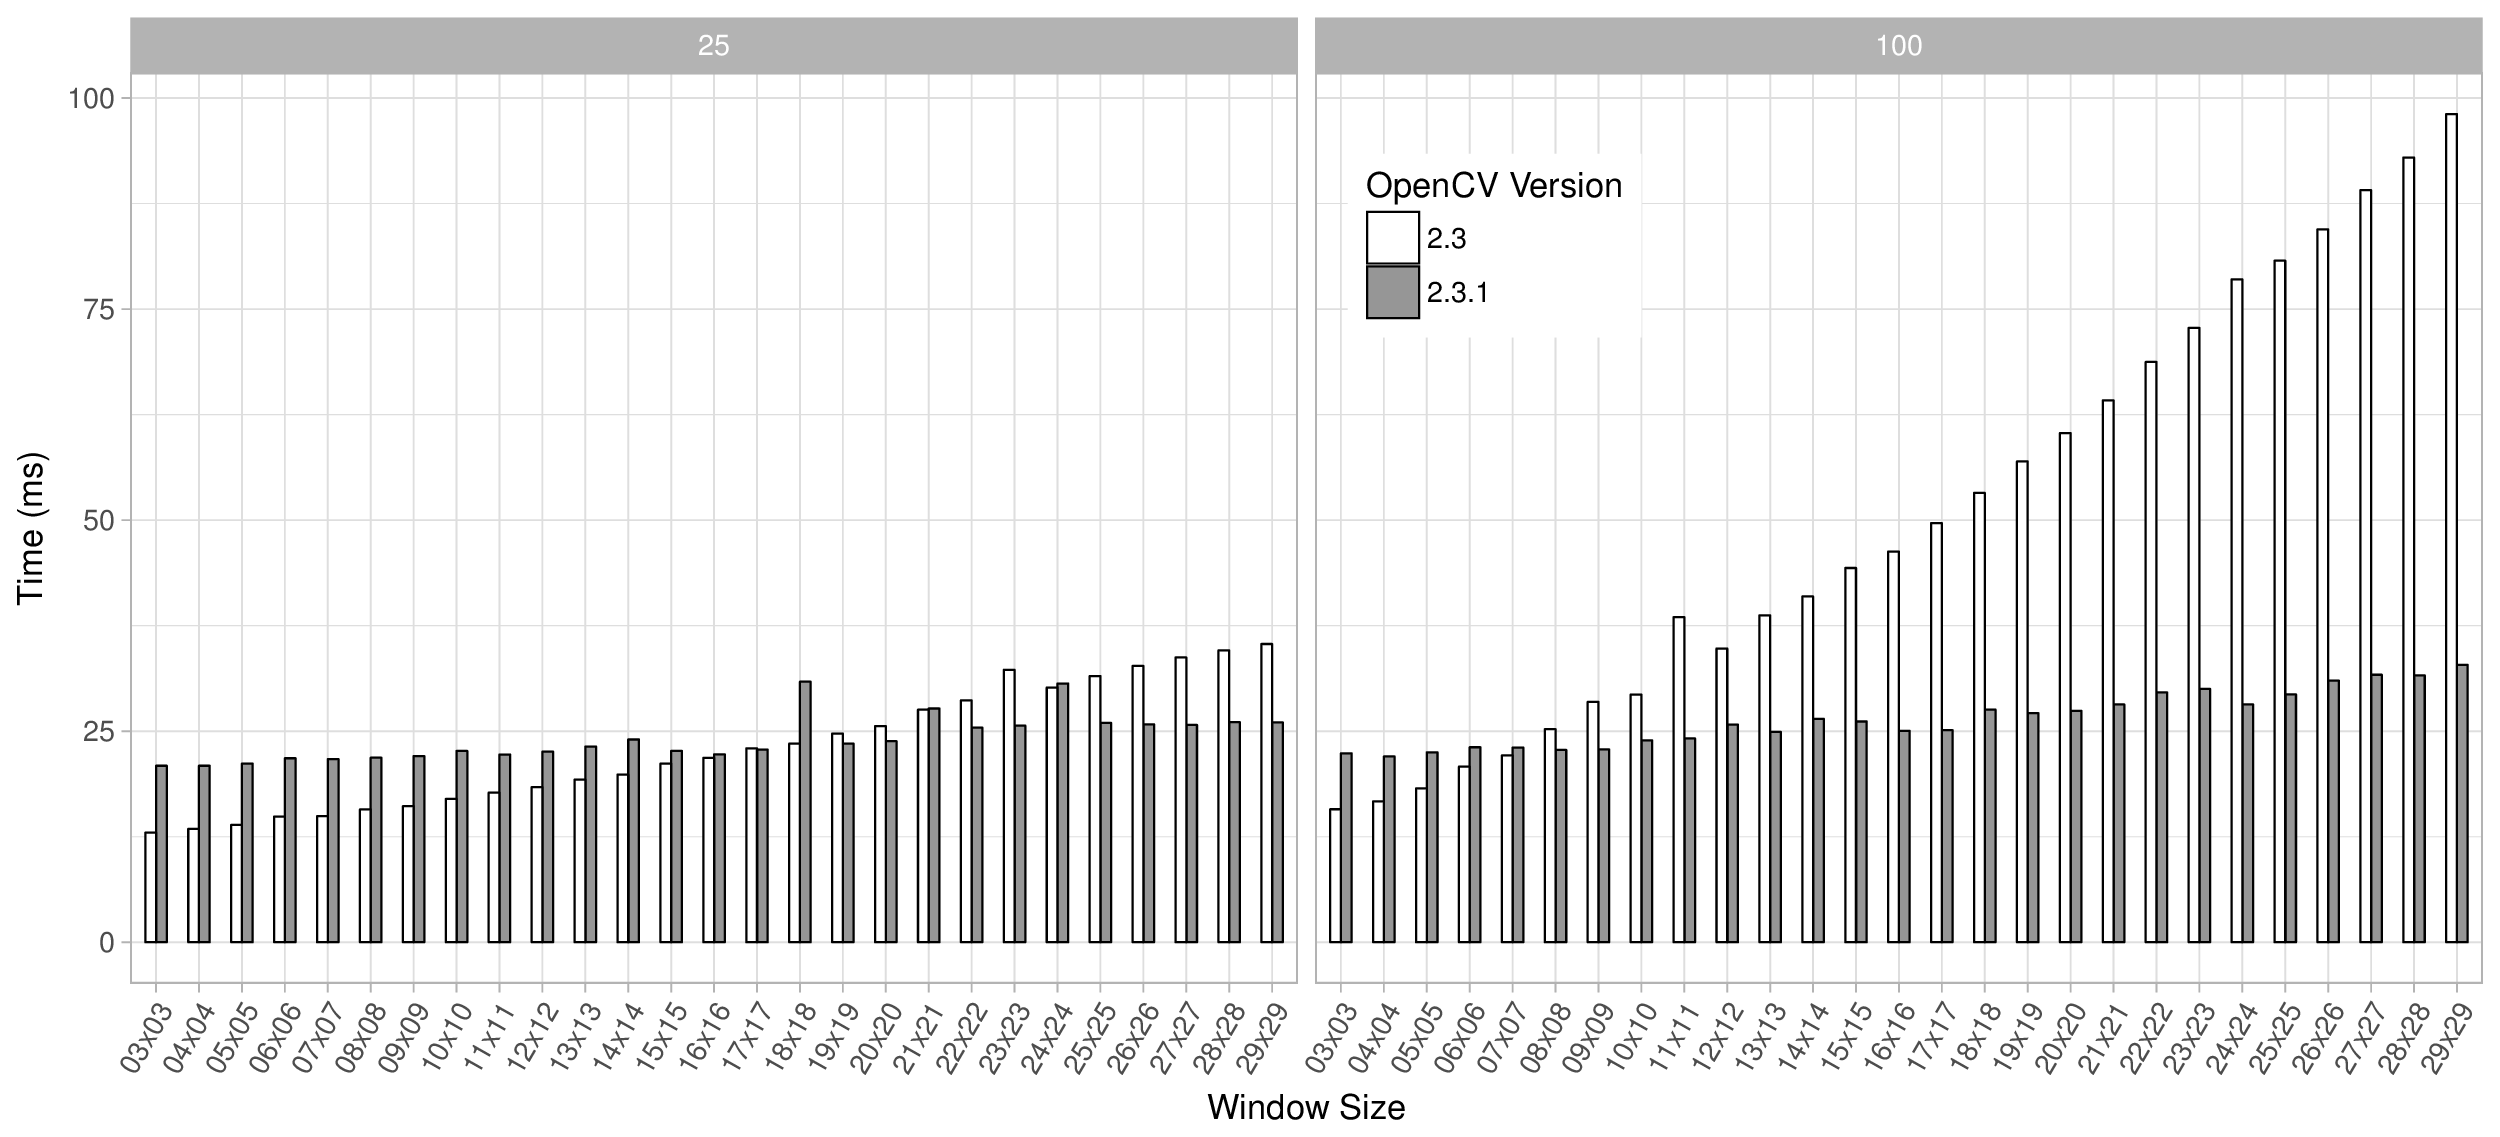
\includegraphics[width=1.0\columnwidth]{figures/opticalflow-regressions.png}
    \caption{OpticalFlow Performance Regressions}
    \label{fig:opticalflow-regressions}
    \vspace{-10pt}
\end{figure*}
\subsection{\textbf{OpenCV}}
Open Source Computer Vision Library (OpenCV) is an open source computer vision and machine learning software library. This library is used in different problems in computer vision as tracking image. In this section, we will benchmark Optical Flow and HoughLines algorithms, which they are the most evolving features in the recent years.

\subsubsection{Optical Flow} 
The Optical Flow, implemented as Lucas-Kanade algorithm, is an example of method in OpenCV and aims to correlates the apparent motion of objects between two consecutive frames. From some examples of the book \cite{opencv2_book}, this method can be tested with two images and show differences on them. Regressions can be caused by a series of changes on the code. Doing the tests we found a relevant regression on the function Optical Flow. \\
The Figure \ref{fig:opticalflow-regressions}, explores the regressions in this function, showing the performance of both versions according to the windows size. Interesting to highlight the fact that the performance of the newer version is better than the previous one until a certain point, where the previous version overpass the newer. 

\textbf{Approach}: Our approach was to run the software several times recording performance metrics using Linux Perf Events. The elapsed time to track the performance is also used in the classification. The runs were related with several versions of OpenCV until a regression was found between the versions 2.3.0 and 2.3.1, the latest version was around 5 times slower than others.


\textbf{Results}: Using the approach above described, which the nodes of the tree have the frames of the OpenCV function call. After carefully analyzing the data, the results the nodes of the newer version, considering all the other metrics, had more instructions. So the there was an association between the longer duration with more instructions.\\
Later we verified the existence of a conditional statement different from one version to another, which makes the slower to execute more instructions. This behaviour was originally reported on \cite{regression_opencv}.
The total number of commits on those two versions were about 250 commits, using this technique, it was able to reduce the difference for about few lines of code and unit tests can be made to trigger specifically this cause after knowing that it is a cache misses problem. \\

\begin{table}[h]
\centering
\caption{Correlation among metrics}
\label{tab:metric-correlation}
\begin{tabular}{lcccccl}
\cline{2-6}
\multicolumn{1}{c|}{} & \multicolumn{1}{c|}{inst.} & \multicolumn{1}{c|}{\begin{tabular}[c]{@{}c@{}}cache \\ misses\end{tabular}} & \multicolumn{1}{c|}{\begin{tabular}[c]{@{}c@{}}page \\ faults\end{tabular}} & \multicolumn{1}{c|}{\begin{tabular}[c]{@{}c@{}}sched \\ switches\end{tabular}} & \multicolumn{1}{c|}{prefetching} &  \\ \cline{1-6}
\multicolumn{1}{|l|}{instructions} & \multicolumn{1}{c|}{1} & \multicolumn{1}{c|}{X} & \multicolumn{1}{c|}{X} & \multicolumn{1}{c|}{X} & \multicolumn{1}{c|}{X} &  \\ \cline{1-6}
\multicolumn{1}{|l|}{cache misses} & \multicolumn{1}{c|}{\textbf{0.957}} & \multicolumn{1}{c|}{1} & \multicolumn{1}{c|}{X} & \multicolumn{1}{c|}{X} & \multicolumn{1}{c|}{X} &  \\ \cline{1-6}
\multicolumn{1}{|l|}{page faults} & \multicolumn{1}{c|}{\textbf{0.999}} & \multicolumn{1}{c|}{\textbf{0.956}} & \multicolumn{1}{c|}{1} & \multicolumn{1}{c|}{X} & \multicolumn{1}{c|}{X} &  \\ \cline{1-6}
\multicolumn{1}{|l|}{sched switches} & \multicolumn{1}{c|}{0.022} & \multicolumn{1}{c|}{0.004} & \multicolumn{1}{c|}{0.0004} & \multicolumn{1}{c|}{1} & \multicolumn{1}{c|}{X} &  \\ \cline{1-6}
\multicolumn{1}{|l|}{prefetching} & \multicolumn{1}{c|}{\textbf{0.996}} & \multicolumn{1}{c|}{\textbf{0.969}} & \multicolumn{1}{c|}{\textbf{0.995}} & \multicolumn{1}{c|}{0.014} & \multicolumn{1}{c|}{1} &  \\ \cline{1-6}
 & \multicolumn{1}{l}{} & \multicolumn{1}{l}{} & \multicolumn{1}{l}{} & \multicolumn{1}{l}{} & \multicolumn{1}{l}{} & 
\end{tabular}
\end{table}

In the Table \ref{tab:metric-correlation} the Pearson correlation (R) of the variables is presented, which shows that many metrics are directly proportional, i.e. R bigger than 0.75. This mean that the development of models using those metrics, for example linear or multilinear models, is not adequate and consequently the comparison of groups, in a pair-wise approach, can be applied.

Figure \ref{fig:caseOpt}, shows the tested image of the optical flow from two images. 

\begin{figure}[h]
      \centering
        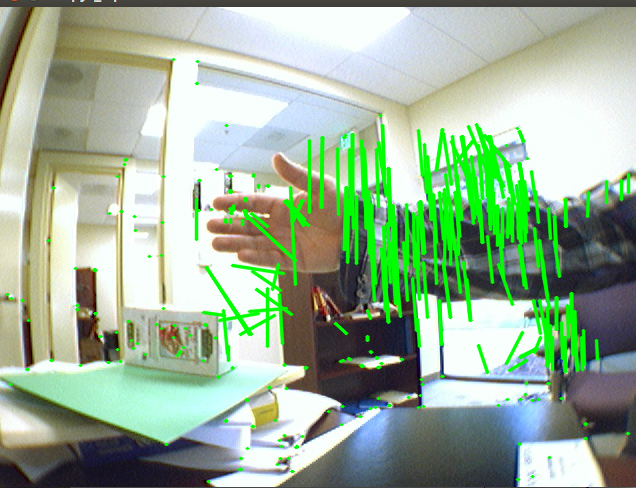
\includegraphics[width=0.45\textwidth]{figures/flow.png}
        \caption{Optical Flow Example}
        \label{fig:caseOpt}
        \vspace{-5pt}
\end{figure}


\subsubsection{HoughLines} 
HoughLines is a line detection mechanism implemented in OpenCV, to find edges in images. This can be used to find edges in roads and it is implemented algorithm is called Canny86. While comparing different versions of opencv, we found that version 3.1 takes more time than version 3.0. in a case of Software Regression \cite{timeTests}. The source code difference can be found here \cite{opencv_source_diff}.

\textbf{Approach}: Our approach was to run the performance unit test several times recording performance metrics using Linux Perf Events in a large file. The elapsed time to track the performance is also used in the classification. The runs were related with several versions of OpenCV until, we found the regression between the versions 3.0 and 3.1, where the newer version was slower than the previous one.


\textbf{Results}: The results correlate the longer duration associated the longer runs with cache misses. By analyzing the code we were able to find a difference on the file hough.cpp, related with a difference size of the called array. This process reduced considerably the search for the causation, helping in the development of a solution.
    
    Figure \ref{fig:case2}, shows the grouping results relating the cache misses with the slow executions groups.
    
    \begin{figure}[h]
          \centering
            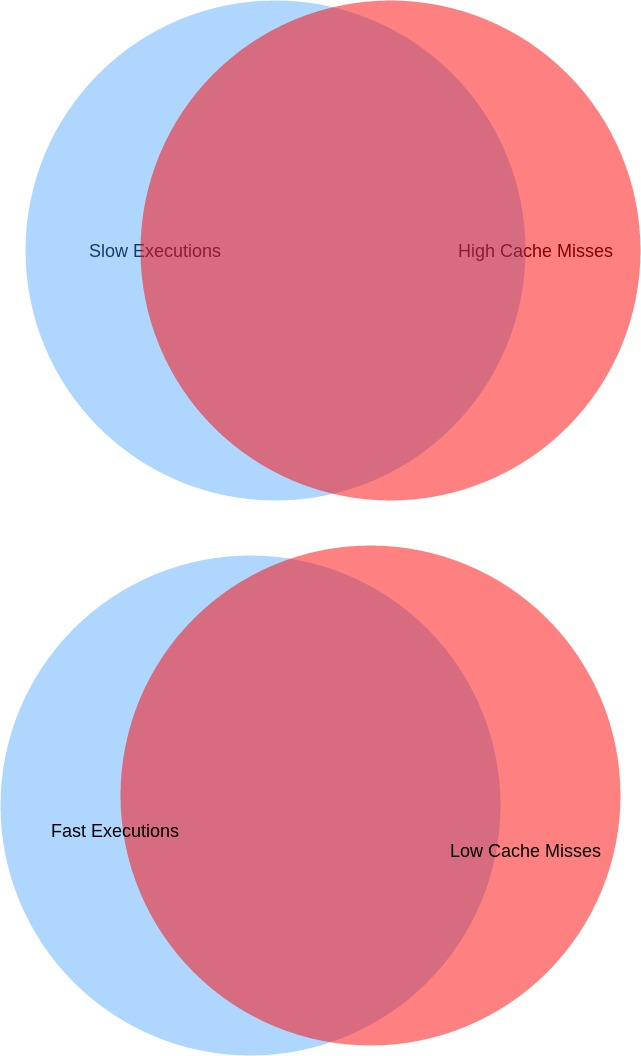
\includegraphics[width=0.350\textwidth]{figures/set_results_cache.jpg}
            \caption{Case study Regression - showing significantly differences in the groups of runs in terms of metrics.}
            \label{fig:case2}
    \end{figure}
    
% The Figure \ref{fig:k-means} shows the use of k-means with 2 as k number of groups.

%     \begin{figure}[h]
%           \centering
%             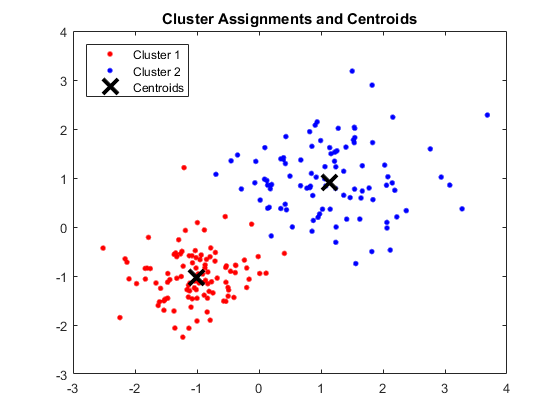
\includegraphics[width=0.50\textwidth]{figures/k-means.png}
%             \caption{K-means result}
%             \label{fig:k-means}
%     \end{figure}
    